%XeLaTeX
\documentclass{article}
\usepackage{lscape}
\usepackage{fontspec}
\setmainfont{DejaVu Serif}
%\newfontfamily{\arm}[Script=Armenian]{DejaVuSans}
\newfontfamily{\arm}[Script=Armenian]{DejaVuSerif-Bold}
\newfontfamily{\armitalic}[Script=Armenian]{DejaVuSerif-BoldItalic}
%\newfontfamily{\arm}[Script=Armenian]{DejaVuSans-Bold}
%\newfontfamily{\armitalic}[Script=Armenian]{DejaVuSans-BoldOblique}
\defaultfontfeatures{Scale=MatchLowercase}
\usepackage[dvipsnames]{xcolor}
\usepackage{eso-pic,graphicx}
\usepackage[top=35mm, bottom=37mm, outer=27mm, inner=27mm, landscape]{geometry}
\color{White}
\renewcommand*\contentsname{\arm{Բովանդակության աղյուսակ}}
\usepackage{fancyhdr}
\pagestyle{fancy}
\fancyfoot[C]{\arm{\thepage}}
\fancyhead{}
\setlength{\emergencystretch}{50pt}
\AddToShipoutPictureBG{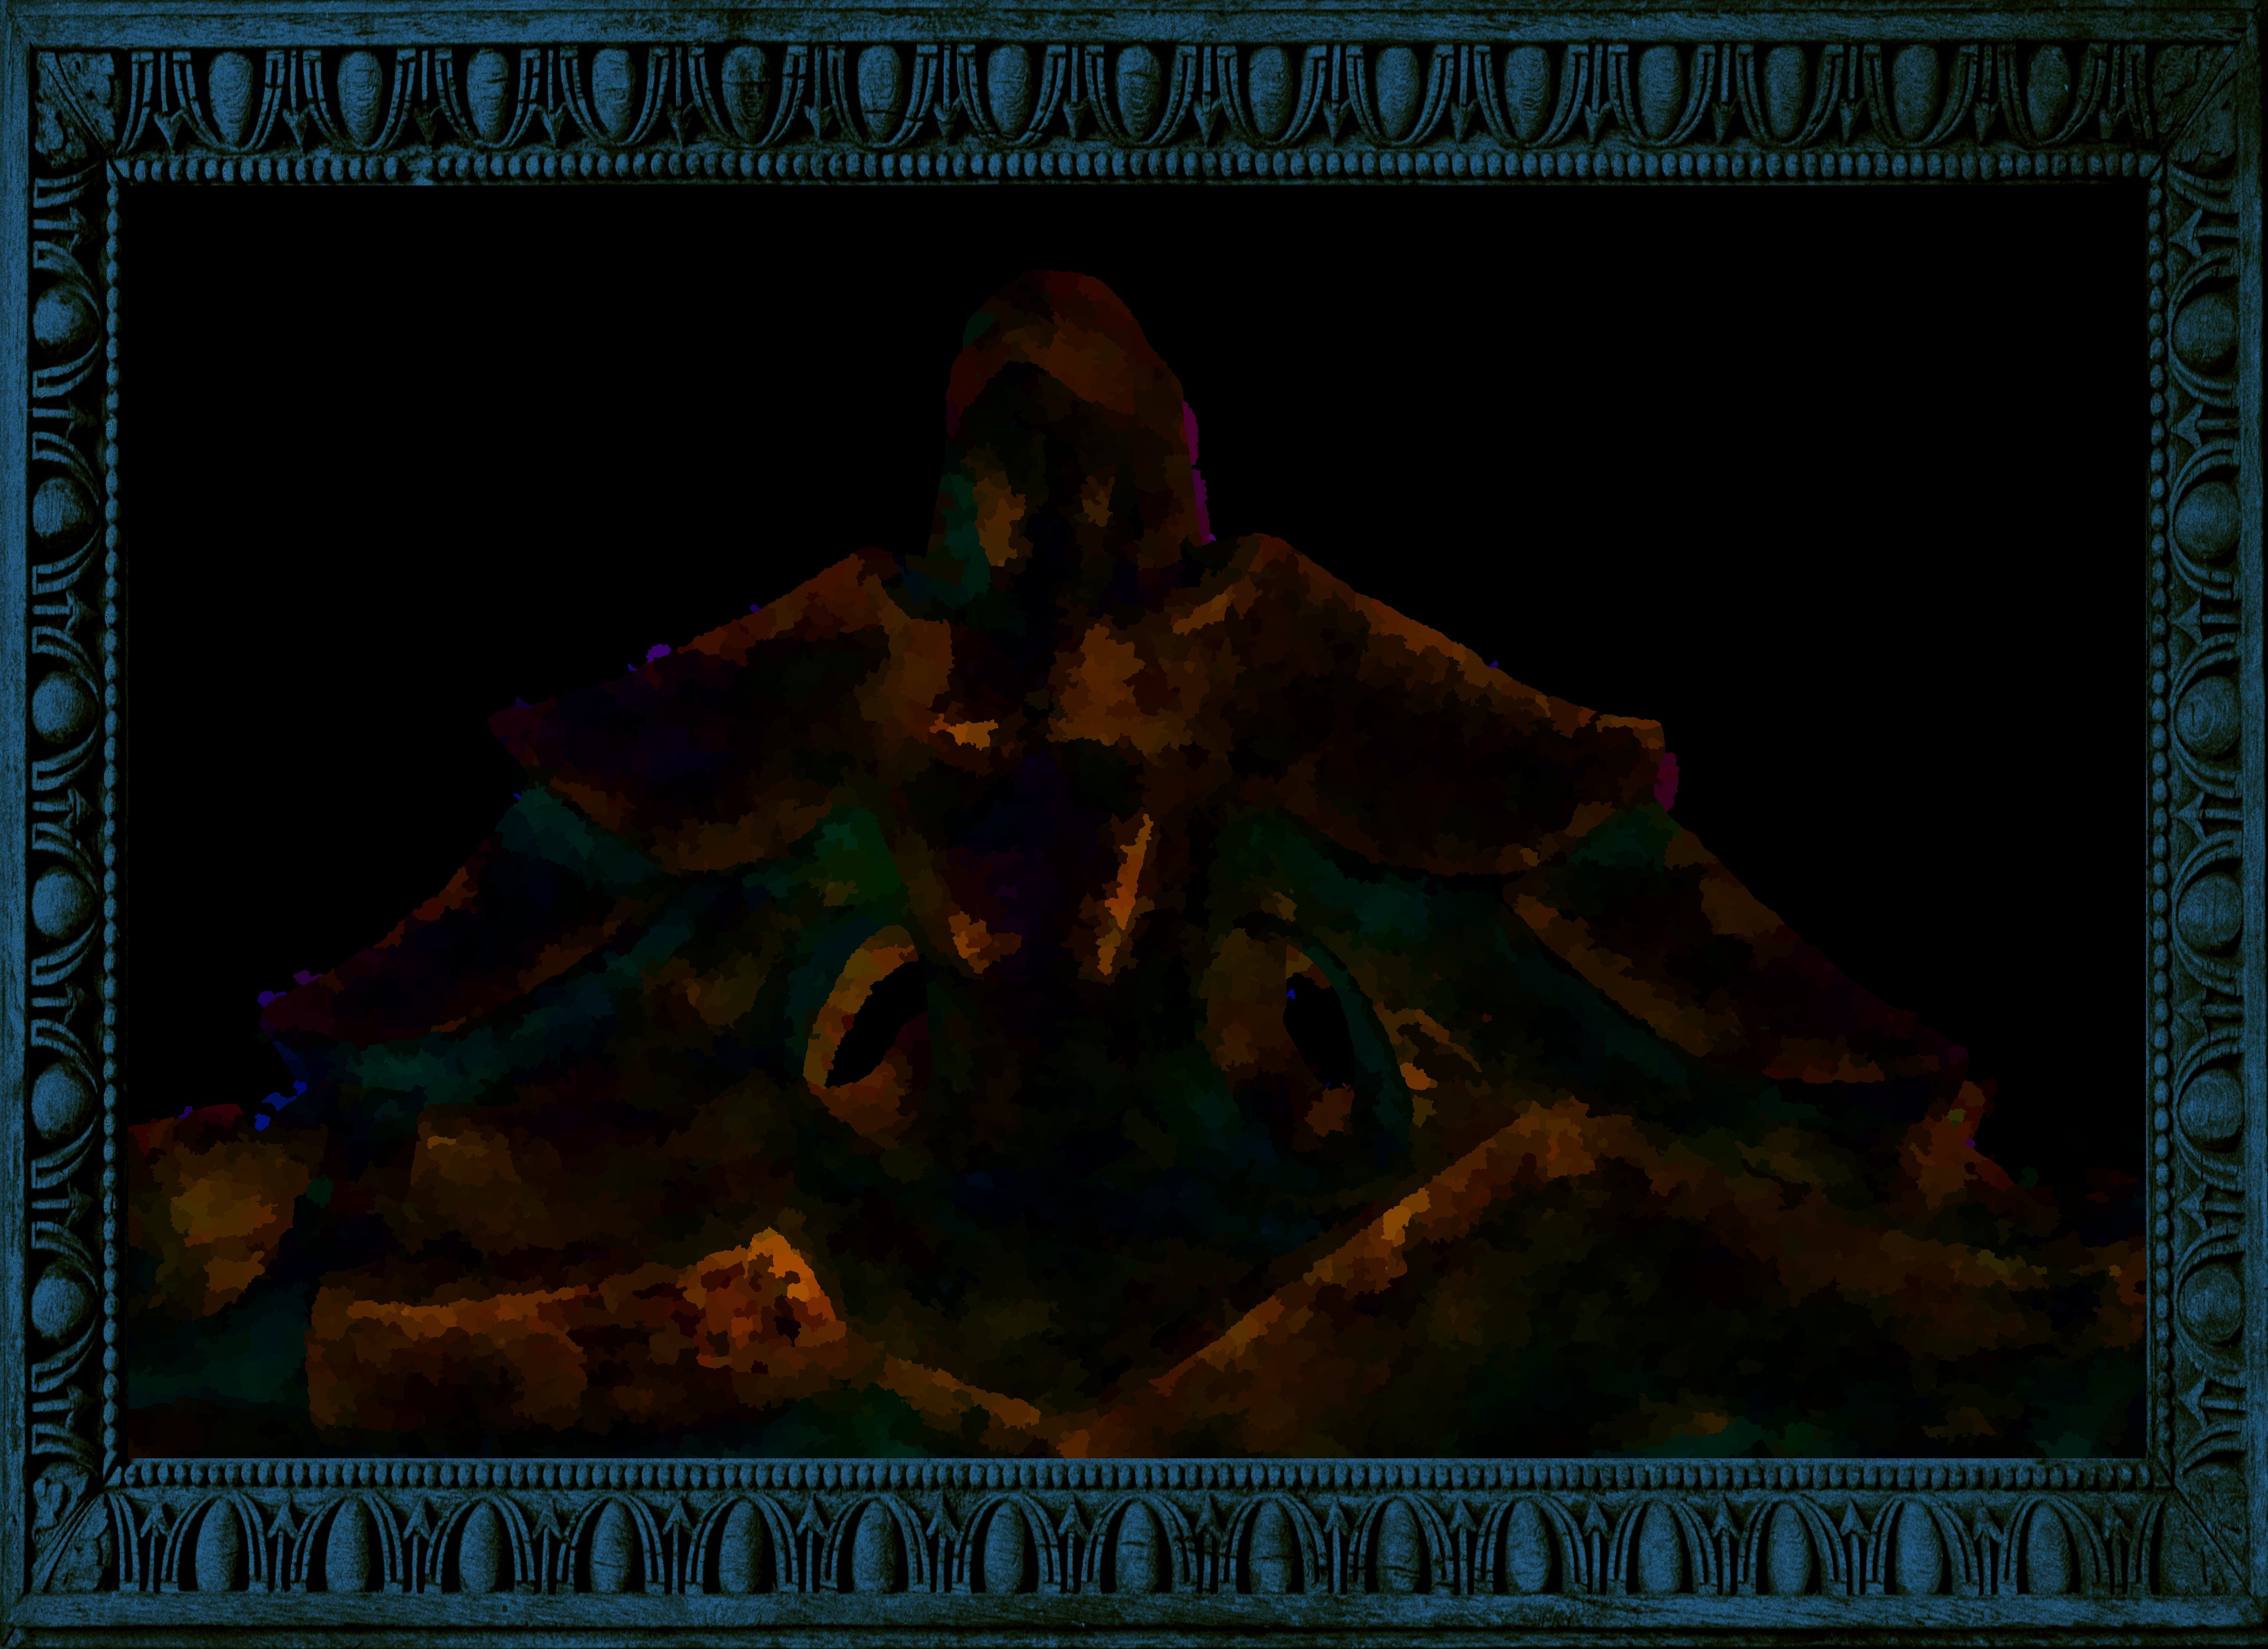
\includegraphics[width=\paperwidth,height=\paperheight]{ara.jpeg}}
\begin{document}

\begin{titlepage} % Suppresses headers and footers on the title page
	\centering % Centre everything on the title page
	%\scshape % Use small caps for all text on the title page

	%------------------------------------------------
	%	Title
	%------------------------------------------------

	\rule{\textwidth}{1.6pt}\vspace*{-\baselineskip}\vspace*{2pt} % Thick horizontal rule
	\rule{\textwidth}{0.4pt} % Thin horizontal rule
	
	\vspace{1\baselineskip} % Whitespace above the title
	
	{\scshape\Huge \arm{Արայ Գեղեցիկ}}
	
	\vspace{1\baselineskip} % Whitespace above the title

	\rule{\textwidth}{0.4pt}\vspace*{-\baselineskip}\vspace{3.2pt} % Thin horizontal rule
	\rule{\textwidth}{1.6pt} % Thick horizontal rule
	
	\vspace{1\baselineskip} % Whitespace after the title block
	
	%------------------------------------------------
	%	Subtitle
	%------------------------------------------------
	
        {\large \arm{Գրեց Հ․ Աղեքսանդր Վ․ Մատիկեան}}
 
        \vspace{1.0\baselineskip}
‌
	%------------------------------------------------
	%	Editor(s)
	%------------------------------------------------
        \vspace*{\fill}    

        \vspace{1.0\baselineskip}

        { \arm{Մխիթարեան տպարան}}
        
	\vspace{1\baselineskip}

        {\small\arm{Վիեննա} 1930}
		
	\vspace{0.25\baselineskip} % Whitespace after the title block

        {\scshape\small \arm{Solar Anamnesis Edition}}% Publication year}
    
	{\scshape\footnotesize \arm{Attribution-ShareAlike 4.0 International }} % Publisher
\end{titlepage}
\clearpage
\tableofcontents
\clearpage
\large
\section*{\arm{Յառաջաբան}}
\paragraph{}
\armitalic{Ներկայ Ուսումնասիրութիւնս, որ 1923էն ի վեր «ՀԱՆԴԻՍԻ» մէջ պարբերաբար հրատարակուեցաւ, ցաւալի է, որ ինծմէ անկախ պատճառներով հազիւ այսօր կրնամ հրապարակ հանել։ Թէեւ յապաղմամբս գործը իր միութենէն ոչինչ տուժած է, սակայն դժբախտաբար նոյնը չէ կարելի հաստատել նաեւ տպագրական թերթերուն թուղթին միօրինակութեան նկատմամբ, որոնց իւրաքանչիւրը կարծես պաշտօնը ստանձնած ըլլար Աւստրիոյ տնտեսական տագնապին դրոշմը կրելու իրենց ճակտին։ Տպագրական ուղղեւիքներու աոանձին ցանկ մը կաղմել հարկ չեմ տեսներ․ միայն մտադիր կ՚ընեմ որ տպագրական 12րդ թերթը մամլոյ տակ դնելու միջոցին սխալմամբ տողերու ետեւառաջութիւն տեղի ունեցած ըլլալուն՝ էջ 179֊180 իմաստի բաւական մեծ խանգարում մտած է․ «ՀԱՆԴԻՍԻ» մէջ արդէն անգամ մը ուղիղ տպուած նախնականը ստանալու համար պէտք է էջ 179֊ի կերջին տողը յաջորդ էջին 5րդ տողէն կերջը զետեղել․ յետոյ էջ 6ի «Պղատոմէնի քով»ը կարդալու է «Պղատոնի քով։»

Հոս պատշաճ կը համարիմ յիշատակել երկու գործեր, որոնք ուսումնասիրութեանս ընթացքին անմատչելի մնացին ինծի․ մին է Արարատ Ամսագիր, Էջմիածին 1918, ուր Լ․ Մելիքսէթ Բեկեան Արալէզներու հայող «Մի՛ քանի խօսք Առլեզի պաշտամունքի մասին» անունով յօդուած մը հրատարակած է․ իսկ միւսն է Dr. Bleichsteiner, Kaukasische Forschungen, 1. Teil, Georgische und Mingrelische Texte, Wien 1919։ Առաջնոյն մէջ Մելիքսէթ Բեկեան կը խօսի Աբխազներու «Ալըշկինդր» շնաստուածներու մասին եւ զրոյց մըն ալ կը հրատարակէ, ուր իբր հերոս կը ներկայանայ Ասլան, որ «բոլոր դեւերը կը սպաննէր․ «Օր մը գողունի կերպով մօտեցան եւ կապեցին մետաքսէ ժապաւէններով եւ կուրացընելով՝ սպաննեցին նրան եւ ձգեցին խորը ջրհոր փոսի մէջ։ Երբ նրա շները վերադարձան, փնտռեցին իրենց տիրոջը, բայց չկարողացան հանել ջրհորից։ Շները երեք օր երեք գիշեր լիզում էին Ասլանին, որի վերադարձրին ե՛ւ կեանքը ե՛ւ տեսողութիւնը․» անդ 125-126։ Այս հետաքրքրական զրոյցին նման նիւթով կը զբաղի նաեւ Dr. Bleichsteinerի թարգմանութեան հրատարակած «Երկու եղբայրներ» անունով վրական զրոյցը, որ սակայն աւելի սերտ աղերսի մէջ կ՚երեւայ ուսումնասիրութեանս էջ 32-40 ներկայացուած Քոյր եւ եղբայր զրոյցին հետ։ Dr. Bleichsteinerի գործը երբ ձեռքս անցաւ, իմ հրատարակածս արդէն տպուած էր։ Ջրոյցը երկու մասի կը բաժնուի, որուն երկրորդ մասը յաւելուած է իմ կարծիքովս։ Առաջին մասն է բուն հետաքրքրականը, որ ընդհանրապէս հետեւեալն է․ Այրի մը որդի մ՚ունէր, որ որսի ժամանակ տեսնելով որ գոմէշ մը եւ անոր ձագը վագրէ մը գիշատուելու վրայ են, կը յարձավի եւ վագրը կը սպաննէ։ Գոմէշը ասոր վրայ շնորհակալ կ՚ըլլայ տղուն եւ իբր վարձք իր ձագը կու տայ անոր Քիչ ատենէն տղան կը տեսնէ, որ փոքրիկ գոմէշը հրաշալիք մըն է ահագին ուժով եւ ամէն բանի կարող։ Անոր վրայ նստած օդոյ վրայէն թռչելով կու գայ կը հասնի մինչեւ ծով մը, զոր վ՚անցնի ու դեւերու թագաւորութեան տէր վ՚ըլլայ։ Բայց իր սխալովը գոմէշը ծովէն ելած վիշապաձգէ մը կը սպաննուի, որ վերջին շունչը չտուած՝ հերոսին կը հրամայէ, որ իր միօը ուտէ, որպէս զի անով իր ոյժը ստանայ եւ ոսկրներն թաղէ, որոնցմէ երկու շնիներ յառաջ կու գան։

Յետոյ կ՚երթայ մայրը կը բերէ, որ վիշապաձկէն խաբուելով՝ տղան սպաննել կ՚ուզէ։ Իմ հրատարակած զրոյցիս պէս հոս ալ հերոսին կեանքին դարանակալը (հոօ մայրը) երեք անգամ հիւանդ կը ձեւանայ եւ առողջանալու համար տղան դժուարին ձեռնարկութիւններու կը մղէ, որոնք ի հարկէ իմ հրատարակածէս քիչ մը տարբեր են։ Առաջին անգամուն մայր խոզ մը կ՚ուզէ, երկրորդին՝ սիրամարգ մը եւ եռորդիին՝ անմահութեան աղբիւրէն ջուր։ Միայն վերջնոյս առթիւ հերոսը Մցիս-Ունախավի (=արեւէն չտեսնուած) աղջկան կը հանդիպի, որ զինքն կը զգուշացընէ, բայց նա միտ չի դներ․ ասոր վրայ աղջիկը կախարդական գաւազան մը կու տայ իրեն, որով լեռը երկուքի կը ճեղքէ եւ անմահութեան ջուրէ կ՚առնու, բայց անկից դառնալու միջոցին՝ շնիկները փակուած կը մնան։ Մայրը ճարահատ տղուն ոյժը փորձել կ՚ուզէ՝ շղթայով մը ձեռքերը կապելով, երբ չոռորդ անգամուն տղղան չորեքպատիկ շղթան ա՛լ չի՛ կրնար խզել, հոն առանձին տեղ մը պահուըտած վիշապաձուկը դուրս ցատկելով զինքն սպաննել կ՚ուզէ, բայց նոյն միջոցին շնիկներն կու գան եւ իրենց տէրը շղթաներէն կ՚ազատեն եւ վիշապը պատառ պատառ կ՚ընեն։ Երկու զրոյցներուն համեմատական նմանութիւնները այնչափ զգալի են եւ յայտնի, որ այս մասին մանրամասնութիւններու իջնալ աւելորդ կը նկատեմ եւ յառաջաբանի մը սահմանէն ալ դուրս։

Գործին ամբողջութեան համար եղած այս երկու փոքրիկ յաւելումներուն կը կցեմ նաեւ ուրիշ կէտ մը, որ ըստ ինքեան իմ մտադրութենէս վրիպած փոքրիկ սխալանք մըն է․ այսինքն՝ էջ 233ին «Ատտիսի առասպելէն յայտնի կ՚երեւայ, որ նաեւ Կիւբեղէ Ատտիսի ծննդականը չի գտներ» խօսքը իր այս ընդհանուր եւ բացասական իմաստով ճիշտ չէ, վասն զի՝ ինչպէս յետոյ մտադիր եղայ ուրիշ տարբերակի մը համաձայն (Arnobius, 5. 14) դիցուհին անդամը ոչ միայն կը գտնէ, այլ եւ առանձին արարողութեամբ ալ կը թաղէ։ Թէեւ գիտնականներէն շատերը ինչ ինչ տեսակէտներով Առնոբիոսի դիցաբանական տեղեկութիւններուն ընդհանրապէս կասկածով կը մերձենան, բայց՝ որչափ կ՚երեւայ, իր ըսածները գէթ ինչ ինչ քաղաքներու համար որոշ հիմ մ՚ունին։

«Նիւթերու եւ անուններու ցանկ ին մէջ առնուած են ինչ որ դիցաբանօրէն նշանակութիւն մ՚ունի ուրիշ կարգի նիւթերէ միայն կարեւորները։»

\bigskip

Հեղինակը
}
\clearpage
\section*{\arm{Ներածոիթիին}}
\paragraph{}
\arm{
«Կրօնի ծագումը եւ դիցաբանութիւն» ուսումնասիրութեան մէջ տուած խոստումս է, որ առաջիկայովս կը կատարեմ։ Նոյն աշխատութիւնը գրելով ուրիշ նպատակ չունէի, բայց եթէ՝ թէ՛ կրօնի եւ թէ՛ դիցաբանութեան մարդկային հոգեկան կեանքին մէջ իւրապատշաճ տեղն տալէն յետոյ բնորոշել առանձնապէս դիցաբանութեան էութիւնն ու նկարագիրը եւ քանի որ վերջինս մեծ մասով նախամարդուն աշխարհահայեացքին հետ կը նոյնանայ, մատնանիշ ընել նաեւ այն աշխարհահայեացքն, որ նախապատմական շրջանին մեր ազգին մէջ կը տիրէր։ Ցորչափ որ այս կարեւոր խնդիրն իւր գէթ ընդհանուր գծերուն մէջ պարզուած չէր, անհնարին էր մեզի հայ պատմութեան մերձենալ, զայն քննել եւ իբր պատմական-գործարանաւոր ամբողջութիւն մը ընթերցող հասարակութեան ներկայացընել։ Վասն զի ամէն ազգային պատմութիւն դիցաբանական աշխարհահայեացքով մը սկսած է․ հետեւաբար մեր անցեալն ալ իր կեանքի բազմապիսի եւ բազմերանգ թելերովը պէտք է որ երթայ ամփոփուի դիցաբանկան շրջանի մը վրայ։ Հոն առաջին անգամ հայ մտքին արեգակը կը ծագի եւ հայ հոգին աղբիւրի մը պէս դուրս կը ժայթքէ մարդկութեան խորքէն։

Այս կէտը հայ պատմաբանի մը մտադրութենէն երբեք վրիպելու չէ․ մեր պատմութեան գորդեան հանգոյցը հոս է․ Աղեքսանդր Մեծին պէս հանգոյցը կտրելով՝ այսինքն հայ դիցաբանութիւնն ըստ մասին անմշակ մէկ կողմ նետելով՝ պատմութիւն գրողները մեզի գեղեցիկ մարմին մը կը ներկայացընեն առանց գլխու եւ առանց գլխու մարմին մը, ինչպէս յայտնի է, կիսով չափ անճանաչելի է։ Անոր համար ալ մեր առասպելական երբեմնի վեհ դէմքերը կը ներկայացուին առ հասարակ կամ որպէս բոլորովին անգոյն եւ կենսազուրկ կմախքներ եւ կամ մէյմէկ անիմաստ ցնորքներ, որոնք հայ դիցաբանական հորիզոնն իրենց առեղծուածային բնոյթով լուսաւորելէ աւելի կը մթագնեն։ Ժողովրդական ամենահին բայց եւ կենսունակ կեանքն է զանոնք ծնողն եւ անոնց սկզբնապատճաոը․ նախ այն խորհրդալիր կեանքին լեզուն հասկընալու ենք․ այլազգ դժուարին է ըմբռնել ոչ միայն ինչ որ ազգային եւ օտար մատենագրութիւնը հայ դիցաբանութեան մասին մեզի կ՚աւանդէ, այլ եւ տեսակէտով մը պիտի մնան մեզի համար անլուծանելի շատ մը պատմական հարցեր եւ այն՚ երբեմն նաեւ շատ կարեւոր հարցեր։ Հարկ կայ յիշեցընելու թէ այն առասպելներ ծնանող եւ կերտող նախապատմութեան հին կեանքը տակաւին բոլորովին մարած շէ․ դարերով շարունակ ազդած է նա մեր մշակոյթին վրայ եւ այսօր իսկ անոր աղդեցութիւնը կարծուածէն աւելի մեծ է։ Քաղաքակըրթութեան տերեւներով եւ դալարագեղ կանանչութեամբ ծածկուած մարդկային սովորական տեսութենէն՝ կը վազէ նա անարգել պղպջուն առուակի մը պէս ժամանակի յարափոխ հովիտէն եւ երբեմն ալ յանկարծ դուրս կ՚ելլէ իւր խոր անկողնէն՝ ցուցընելու համար թէ ինքը դեռ կ՚ապրի, թէպէտ ոչ այնչափ վճիտ եւ կենսունակ, ինչպէս յառաջ, բայց եւ կ՚ապրի եւ կ՚իշխէ հայ ժողովրդեան սրտին ամենաթաքուն խորշերուն վրայ։ Ե․ Լեման բնաւ չի ծայրայեղեր երբ իր Հայաստան ըրած ճամբորդութեան տպաւորութիւնները Archiv für Religionswissenschaft\footnote{\arm{1903, 1., 1։}} թերթին մէջ հրատարակած միջոցին կը յայտարարէ թէ Հայերը իբրեւ քրիստոնեայ շատ խիստ են եւ հաւատարիմ, բայց իրենց շատ մը բարքերով եւ հայեացքներով հեթանոս Հայէն տարբերութիւն չունին։

Վերը յիշուած աշխատութիւնը կարդացողը դիւրաւ պիտի համոզուի հոս ըսուածներուն ճշմարտութեան։ Անդրագոյն զօրաոր ապացոյցներ պիտի մատակարարէ նաեւ առաջիկայ ուսումնասիրութիւնս, որ առաջնոյն բնական մէկ հետեւութիւնն է։ Արայ Գեղեցիկը մեր դիցաբանական շրջանին ամենակարկառուն դէմքերէն մէկն է որ իր քնքոյշ եւ հմայիչ պատկերովը այնպէս պայծառ կերպով դուրս կը ցայտեցընէ Հայուն խրոխտ բայց եւ մաքուր եւ ազնիւ հոգին։ Այս առասպելական դէմքն իբրեւ ճշմարիտ բախտակից մը Հայուն բախտին ընկերացած է հաւատարմօրէն անոր քայլերուն ուր որ ալ գացած է նա․ ինքն ալ ձգած է անոր հետ իր հին հայրենիքը, շրջած է դարերով երկրէ երկիր մինչեւ այն վայրկեանը, երբ մեր նախնիներն իրենց շրջուն կեանքին վերջ դնելով տեղաւորուեցւն վերջնականապէս հնութեան ամենանշանաւոր գետերուն՝ Եփրատի եւ Տիգրիսի կեանք տուող մայր երկրին վրայ, գրաւուելով անոր բիւրազգի աղբիւրներով ոռոգուած կանանչազարդ ծաղկապսակ հովիտներէն եւ չքնաղ գեղեցկութեամբ պճնուած երկնաբերձ հսկայ լեռներէն, որոնք օտար ասպատակութիւններու պահուն կրնային իրենց ամուր ապաստանարանի դեր ալ կատարել։ \emph{Արայ Գեղեցիկն ուսումնասիրել կը նշանակէ հայ ազգին ծագման մթին դարերը թեւակոխել եւ քննել։} Եւ ինչ զարմանք, եթէ Հայուն հետ նաեւ առասպելս մեծամեծ փոփոխութիւններու ենթարկուած է դարերու ընթացքին, այն աստիճանի որ շատ մը գիտնականներ մինչեւ անգամ անոր հայկական նկարագիրը կամ բոլորովին եւ կամ ըստ մասին ուրացան եւ ասորական ապրանք մը նկատեցին։\footnote{\arm{Եր․ Տէր-Մինասեան․ Բաբելոն եւ Սուրբ գիրք, Յաւելուած Գիլգամեշի վեպը, Վաղարշապատ, 1908. — Բասմաջեան․ Իսկական պատմութիւն Հայոց, Պոլիս, էջ 81-82. — նաեւ՝ Համեմատական հետազօտութիւն մեր Յարալիզաց եւ Բաբելացւոց Մերովդաքի, վենետիկ 1898։}} Հայերն ալ երբեմն սեմական՝ ոմանցմէ ալ տուրանեան նկատուեցան իրենց մարդախօսական կազմին ինչ ինչ յատկութիւններուն պատճառաւ։ Սակայն քննութիւնը հոս շուտով մթութեան վարագոյրը վերցուց եւ ճշմարտութիւնն երեւան բերաւ։ Կը յուսանք թէ Արայի առասպելն ալ, որ մեր դիցաբանութեան բեկորներուն ամէնէն ազնիւ գոհարն է կրնանք ըսել, ուրիշ բախտի պիտի չարժանանայ։ Գրութեանս նպատակն է անոր հայկական նկարագիրն ոչ միայն փրկել, այլ աւելի եւս յառաջ երթալով փորձել ցուցընելու թէ առասպելս իր ամենանախնական ձեւին մէջ հնդեւրոպական մայր-աղբիւրէն կը բխէ եւ հետեւաբար՝ հնբեւրոպական ազգերու գէթ որոշ մէկ խմբին հասարակաց աշխարհահայեացքին մէկ մասը կը կազմէր։

Մեր անմիջական գործը պիտի ըլլայ նախ եւ յառաջ Արայի մասին եղած ազգային գրական աւանդութիւնը քննութեան բովէ անցնել, զտել, մաքրել ինչ որ յաւելուած է մատենագիրներու կողմանէ եւ իրեն չի վերաբերիր մէկ խօսքով մատնացոյց ընել գէթ աղօտ կերպով այն առասպելն, որ Դ-Երդ դարերու հայ ժողովրդեան հեթանոսական հայեացքներուն գլխաւոր առարկաներէն մէկն էր եւ զինքն կարծուածէն աւելի կը զբաղցընէր։ Սակայն հայ առասպելագիտութեան քիչ թէ շատ ծանօթ գիտնականի մը համար պարզ է թէ Արայի կնճռոտ խնդրոյն համար ազգային աղբիւրներն անբաւական են․ անոր բանալին մեզի բուն իսկ համեմատական քննութիւնը պիտի ընձեռէ, որուն մէջ պիտի աշխատինք համեմատական նոյնօրինակ առասպելներով լուսաւորել ինչ որ ազգային աղբիւրները մթին կը թողուն, ամբողջացընել պակասը եւ հետեւիլ պատմական այն յառաջատութիւններուն, որոնցմէ անցած է Արայ Գեղեցիկը մինչեւ որ Երդ դարուն իր վերջնական կերպարանքն ստացաւ։ Այս համեմատական քննութեան պիտի յաջորդէ աւելի մասնական եւ այն շատ շահագրգռական հարց մը, այսինքն՝ Արայ Գեղեցիկը Պղատոմէնի քով․ ամէնուն պսակը պիտի կազմէ հետահայեաց ակնարկ մը ամբողջին վրայ, ուր պիտի աշխատինք նաեւ Արայի անուան դժուարին հարցը լուծել։
}
\clearpage
\section{\arm{Աջգային Աղբիիրներ Արայի Մասին}}
\subsection{\arm{Գրական աւանդութիւն}}
\paragraph{}
\arm{Արայի աւանդավէպին վրայ խօսող երեք գլխաւոր աղբիւր ունինք՝ Անանուն, Եզնիկ եւ խորենացի, որոնց մէջէն կարեւորագոյնն առանց տարակուսի Անանունն է․ այն խորհրդաւոր թաքուն հեղինակն, որ ուրիշ կողմանէ մեզի Փաւստոս անուամբ ալ ծանօթ է։\footnote{\arm{Հմմտ․ Հ․ Ա․ Մ[?], Անանունը կամ Կեղծ Սեբէոս, Վիեննա 1913 (Ազգ․ Մատենադր․ Թ․ 70)։}} Եզնիկ թէել առասպելիս մասին մեզի քանի մը շատ հետաքրքրական մանրամասնութիւններ կը հաղորդէ, բայց ամբողջ խնդիրն աւելի հարեւանցի կը շօշափէ, իսկ խորենացին, յարգելով հանդերձ իր ուրիշ շատ մը բարեմասնութիւններն, հոս գրեթէ ստրկօրէն Անանունի հետեւելով չունի այսօր այլ եւս այն արժէքն ու նշանակութիւնը, ինչ որ երբեմն իրեն կ՚ընծայուէր։ Մեր խորենացւոյ հանդէպ բռնած այս ընթացքն անշուշտ նորութիւն մը պիտի նկատուի․ անոր համար թերեւս անիրաւ ալ երեւայ կարգ մը գիտնականներու, որոնք խորենացւոյ երբեմնի փառքին փայլէն գրաւուած եւ մասամբ նաեւ յափշտակուած՝ ամէն ճիգ կը թափեն անոր նախնական բարձրադիր գահը փրկելու համար։ Սակայն կը յուսանք թէ հայ պատմախոյզներու եթէ ոչ ամէնքը՝ գէթ մեծամասնութիւնը դանդաղ քայլերով, բայց վերջ ի վերջոյ այն համոզման պիտի գայ որ հայ \emph{առաջին պատմագիրը, հայ հերոդոտոսը Խորենացին չէ, ինչպէս ընդհանրապէս կը կարծուի, այլ Փաւստոս}, հնութենէ ընդհանրապէս, բայց ամենէն աւելի ինքնին իսկ խորենացիէն այնչափ անարգուած այն պատմագիրը, որ լայնամիտ հեռատեսութեամբ եւ Երդ դարու մեր ուրիշ մատենագիրներու քով չտեսնուած քաջութեամբ յանդըգնութիւնն ունեցաւ ազգային ամբողջական պատմութիւն մը գրելու, առանց զանց առնլու ազգային հին հեթանոսական հերոսներն ու առասպելներն, որոնց մինչեւ իսկ Եզնիկ հեռուէն միայն մօտեցած է։ Cuique suum սկզբունքը հոս ալ իր արժէքն ունի։ Խորենացւոյ պատմական արժէքն ոչ ոք կ՚ուրանայ, մանաւանդ թէ որոշ կարգի հարցերու մէջ բացարձակ է իր հեղինակութիւնը, բայց ուր որ Անանուն-Փաւստոսի, Ագաթանգեղոսի Կորեան եւ Ղազար Փարպեցւոյ ձայնը լսելի կ՚ըլլայ, հոն պարզապէս արձագանգի դեր կը կատարէ Խորենացին, հետեւող է եւ աշակերտ, հակառակ իր իսկ կամքին եւ բաղձանքին։}
\clearpage
\subsection{\arm{Ժողովրդական աւանդութիւն}}
\paragraph{}
\clearpage
\subsection{\arm{Շամիրամ}}
\paragraph{}
\clearpage
\subsection{\arm{Արալէզները}}
\paragraph{}
\clearpage
\section{\arm{Օտար Աղբիիրներ Արայի Մասին Եի Համեմատոիթիիններ}}
\subsection{\arm{Արայ Գեղեցիկի համապատասխան առասպելներ}}
\paragraph{}
\clearpage
\subsection{\arm{Արայ Գեղեցիկ յոյն մատենագրութեան մէջ}}
\paragraph{}
\clearpage
\subsection{\arm{Արայ անունը եւ իր ծագումը}}
\paragraph{}
\clearpage

\end{document}
